%% img/NPClass/SATdHAM2.tex
%% Copyright 2019 Andrea Berlingieri
%
% This work may be distributed and/or modified under the
% conditions of the LaTeX Project Public License, either version 1.3
% of this license or (at your option) any later version.
% The latest version of this license is in
%   http://www.latex-project.org/lppl.txt
% and version 1.3 or later is part of all distributions of LaTeX
% version 2005/12/01 or later.
%
% This work has the LPPL maintenance status `maintained'.
%
% The Current Maintainer of this work is Andrea Berlingieri.
%
% This work consists of all files listed in manifest.txt
\documentclass{standalone}

\usepackage{../TikzStyle}
\usepackage{../mystyle}
%\usetikzlibrary{decorating}
\usetikzlibrary{positioning}

\newcommand{\Chain}[3]{%
    \node[point] (#3_n1) at ([shift={(#1 cm, #2 cm)}]0,0) {};
    \node[point] (#3_n2) at ([shift={(#1 cm, #2 cm)}]1,0) {};
    \node[point] (#3_n3) at ([shift={(#1 cm, #2 cm)}]2,0) {};
    \node[point] (#3_n4) at ([shift={(#1 cm, #2 cm)}]3,0) {};
    \node[point] (#3_n5) at ([shift={(#1 cm, #2 cm)}]4,0) {};
    \node[point] (#3_n6) at ([shift={(#1 cm, #2 cm)}]5,0) {};
    \draw[->,xshift=#1 cm, yshift=#2 cm] (#3_n1) .. controls (0.25,0.5) and (0.75,0.5) .. (#3_n2);
    \draw[->,xshift=#1 cm, yshift=#2 cm] (#3_n2) .. controls (1.25,0.5) and (1.75,0.5) .. (#3_n3);
    \draw[->,xshift=#1 cm, yshift=#2 cm] (#3_n3) .. controls (2.25,0.5) and (2.75,0.5) .. (#3_n4);
    \draw[->,xshift=#1 cm, yshift=#2 cm] (#3_n4) .. controls (3.25,0.5) and (3.75,0.5) .. (#3_n5);
    \draw[->,xshift=#1 cm, yshift=#2 cm] (#3_n5) .. controls (4.25,0.5) and (4.75,0.5) .. (#3_n6);
    \draw[->,xshift=#1 cm, yshift=#2 cm] (#3_n2) .. controls (0.75,-0.5) and (0.25,-0.5) .. (#3_n1);
    \draw[->,xshift=#1 cm, yshift=#2 cm] (#3_n3) .. controls (1.75,-0.5) and (1.25,-0.5) .. (#3_n2);
    \draw[->,xshift=#1 cm, yshift=#2 cm] (#3_n4) .. controls (2.75,-0.5) and (2.25,-0.5) .. (#3_n3);
    \draw[->,xshift=#1 cm, yshift=#2 cm] (#3_n5) .. controls (3.75,-0.5) and (3.25,-0.5) .. (#3_n4);
    \draw[->,xshift=#1 cm, yshift=#2 cm] (#3_n6) .. controls (4.75,-0.5) and (4.25,-0.5) .. (#3_n5);
}

\begin{document}
    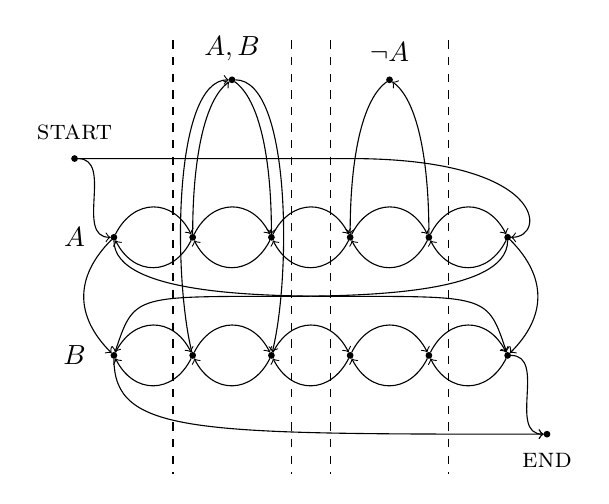
\begin{tikzpicture}[point/.style={draw,circle,inner sep=0cm,fill=black,minimum size=2pt}]
        \node[point] (start) at (-0.5,1) {};
        \node[point] (end) at (5.5,-2.5) {};
        \node () [above=2pt of start] {$\textsc{start}$};
        \node () [below=2pt of end] {$\textsc{end}$};
        \node () at (-0.5,0) {$A$};
        \node () at (-0.5,-1.5) {$B$};
        \Chain{0}{0}{Achain};
        \Chain{0}{-1.5}{Bchain};
        \draw[->] (start) .. controls (0,1) and (-0.5,0) .. (Achain_n1);
        \draw[->] (start) -- (3,1) .. controls (5.5,1) and (5.5,0) .. (Achain_n6);
        \draw[->] (Achain_n6) .. controls (5.5,-0.5) and (5.5,-1) .. (Bchain_n6);
        \draw[->] (Achain_n1) .. controls (-0.5,-0.5) and (-0.5,-1) .. (Bchain_n1);
        \draw[->] (Achain_n1) .. controls (0,-0.75) and (2,-0.75) .. (3,-0.75) .. controls (4.75,-0.75)
        and (4.75,-0.75) .. (Bchain_n6);
        \draw[->] (Achain_n6) .. controls (5,-0.75) and (3,-0.75) .. (2,-0.75) .. controls (0.25,-0.75)
        and (0.25,-0.75) .. (Bchain_n1);
        \draw[->] (Bchain_n6) .. controls (5.5,-1.5) and (5,-2.5) .. (end);
        \draw[->] (Bchain_n1) .. controls (0,-2.5) and (1,-2.5) .. (end);
        \node[point] (ab) at (1.5,2) {};
        \node () [above=2pt of ab] {$\set{A,B}$};
        \draw[dashed] (0.75,2.5) -- (0.75,-3);
        \draw[dashed] (2.25,2.5) -- (2.25,-3);

        \node[point] (na) at (3.5,2) {};
        \node () [above=2pt of na] {$\set{\lnot A}$};
        \draw[dashed] (2.75,2.5) -- (2.75,-3);
        \draw[dashed] (4.25,2.5) -- (4.25,-3);
        \draw[<-] (Achain_n4) .. controls (3,1) and (3.15,1.75) .. (na);
        \draw[<-] (na) .. controls (3.85,1.75) and (4,1) .. (Achain_n5);
        \draw[->] (Achain_n2) .. controls (1,1) and (1.15,1.75) .. (ab);
        \draw[->] (ab) .. controls (1.85,1.75) and (2,1) .. (Achain_n3);
        \draw[->] (Bchain_n2) .. controls (0.75,-0.5) and (0.75,2) .. (ab);
        \draw[->] (ab) .. controls (2.25,2) and (2.25,-0.5) .. (Bchain_n3);
    \end{tikzpicture}
\end{document}
